\selectlanguage{english}

\chapter{Reject Inference} \label{chap2}

\epigraph{Sounds good, doesn't work.}{Donald J.\ Trump}

\minitoc

\textit{Nota Bene :} ce chapitre s'inspire fortement de l'article [...]

\bigskip




\section{Consumer loans: acceptance and financing process}



\begin{figure}[ht]
\begin{minipage}[b]{0.45\linewidth}
\center 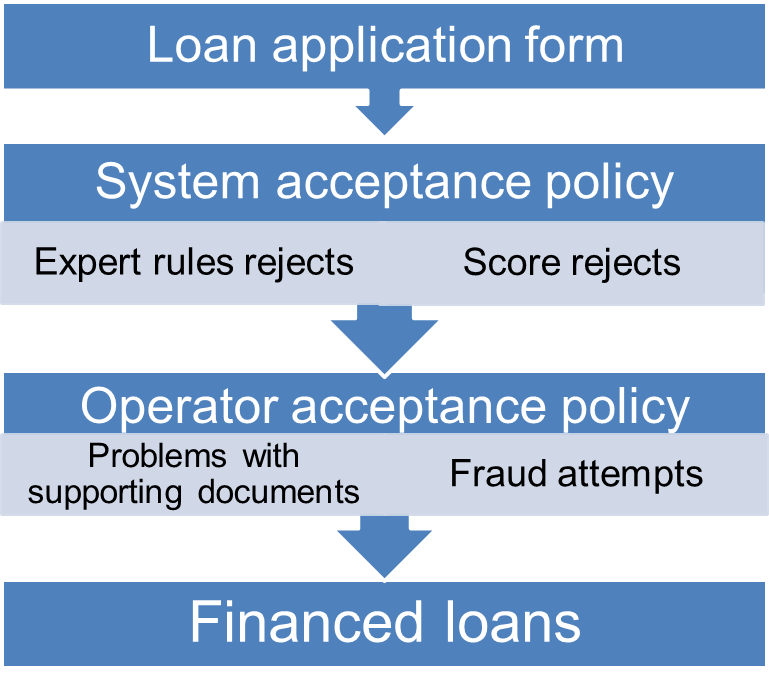
\includegraphics[width=5cm]{figures/chapitre2/schema.png}
\caption{Simplified Acceptance mechanism in~Crédit Agricole Consumer Finance}
\label{fig:figure1}

\end{minipage}%
\hfil \begin{minipage}[b]{0.5\linewidth}

\center 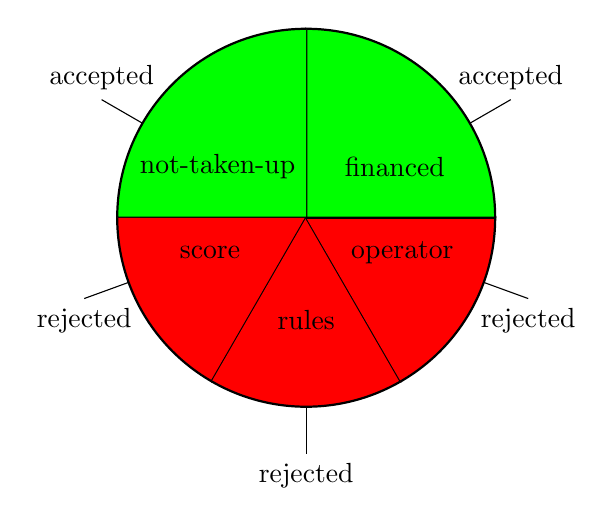
\begin{tikzpicture}

    \foreach \start/\end/\middle/\percent/\anchor/\name in {
      0/90/30/financed/above/accepted,
      90/180/150/not-taken-up/above/accepted}
  {
    \draw[fill=green, thick] (0,0) -- (\end:2.4cm) arc (\end:\start:2.4cm)
      node at (\middle:1.3cm) {\percent};
    \draw (\middle:2.4cm) -- (\middle:3cm) node[\anchor] {\name};
  };
    
    \foreach \start/\end/\middle/\percent/\anchor/\name in {
      180/240/200/score/below/rejected,
      240/300/270/rules/below/rejected,
      300/360/340/operator/below/rejected}
  {
    \draw[fill=red, thick] (0,0) -- (\end:2.4cm) arc (\end:\start:2.4cm)
      node at (\middle:1.3cm) {\percent};
    \draw (\middle:2.4cm) -- (\middle:3cm) node[\anchor] {\name};
  };
\end{tikzpicture}
\caption{Simplified Acceptance status in Crédit Agricole Consumer Finance - scale relations not respected}
\label{fig:figure2}

\end{minipage}
\end{figure}



\printbibliography[heading=subbibliography, title=References of Chapter 2]